%Every LaTeX file needs a documentclass declaration.
%Possibilities are article, book, letter.  Font size is also declared.

\documentclass[10pt]{article}

%special packages used for symbols, formatting, etc.

\usepackage{amsmath} % contains the align* environment, which is great for manipulating formulas
\usepackage{amssymb} % contains common symbols
\usepackage{amsthm} % has the proof environment
\usepackage[margin=1in]{geometry} % specifies page properties, such as the margin
%\usepackage{siunitx} % useful for typesetting units
\usepackage{tikz} % useful for graphics

% Define a lemma environment
% Set the style of the new theorem environments so that the text isn't in italics
\theoremstyle{definition}
% Define lemma environment, the first argument is the name in LaTeX, the second argument is what is typeset
\newtheorem{lemma}{Lemma}

% User-defined commands

\newcommand{\newprob}{\medskip \hrule \medskip}
\newcommand{\fanc}[1]{\mathbb{#1}}
\newcommand{\rn}[1]{\fanc{R}^{#1}}
\def\qed{\hspace*{\fill}\rule{1.854mm}{3mm}}  % the fancy box at the end of a proof

%%%%%%%%%%%%%%%%%%%%%%%%%%%%%%%%%%%%%%%%%%%%%%

%beginning of document, every \begin{} also requires an \end{} command.

%\renewcommand{\baselinestretch}{2}

\begin{document}

\pagestyle{empty}  %suppress page numbers, etc.

\begin{center}  %center command, also see flushright, flushleft

{\bf MATH 423-01  Advanced Calculus I

Homework \#6

Assigned: October 26, 2022

Due: November 2, 2022}

\end{center}

\medskip

\hrule   %horizontal line

\bigskip

% list environment: description, itemize, and enumerate

\begin{enumerate}

%%%%%%%%%%%%%%%%%%%%%%

\item  ~[Hale, A.] Prove the reverse of the theorem that says that a point $x$ is a limit point of a set $A$ if and only if $x = \lim{a_n}$, for some $(a_n) \subseteq A$ such that $x \neq a_n$, $\forall n \in \mathbb{N}$.
\begin{proof}
Assume that $\exists (a_n) \subseteq A$ such that $x \neq a_n, \forall n \in \mathbb{N}$ with $x=\lim{a_n}$.  We need to prove that $x$ is a limit point.  To do this, we need to BLANK.
\end{proof}
	
%%%%%%%%%%%%

%\item  Decided whether the following sets are open, closed, or neither.  If a set is not open, find a point in the set for which there is no neighborhood contained in the set.  If a set is not closed, find a limit point that is not contained in the set.
%
%	\begin{enumerate}
%	
%	\item  $\{x \in \mathbb{R}: x>0\}$
%	
%	\item  $(0,1]$
%	
%	\item  $\{1 + 1/4 + 1/9 + \cdots + 1/n^2: n \in \mathbb{N}\}$
%	
%	\end{enumerate}
	
%%%%%%%%%%%%%%%%

%\item  \begin{enumerate}
%	
%	\item  Give an example of an infinite collection of nested open sets whose intersection, $\cap_{n=1}^{\infty} \Omega_n$, is closed and nonempty.
%	
%	\item  Give an example of an infinite collection of nested closed sets whose union, $\cup_{n=1}^{\infty} F_n$, is open and nonempty.
%	
%	\end{enumerate}
	
%%%%%%%%%%%%%%

\item  ~[Harter, J.] Let $A$ be bounded above so that $s = \sup{(A)}$.  Prove that $s \in \overline{A}$.
	
%%%%%%%%%%%%
	
\item  Decide whether the following statements are true or false.  Provide counterexamples for those that are false and proofs for those that a true.

	\begin{enumerate}
	
	\item  ~[James, J.] For any set $A \subseteq \mathbb{R}$, $(\overline{A})^c$ is open.
	
	\item  ~[James, J.] If a set $A$ has an isolated point, then it cannot be an open set.
	
	\item  ~[James, J.] An open set that contains every rational number must necessarily be all of $\mathbb{R}$.
	
	%\item  If $A$ is a bounded set, then $s = \sup{(A)}$ is a limit point of $A$.
	
	\item  ~[Kline, L.] A set $A$ is closed if and only if $\overline{A} = A$.
	
	\item  ~[Kline, L.] Every finite set is closed.
	
	
	
	\end{enumerate}
	
%%%%%%%%%%%%%

\item  ~[Krason, T.] Decide which of the following sets are compact.  For those that are not compact, show how the definition breaks down: give an example of sequence contained in the set that does not possess a subsequence converging to a limit in the set.

	\begin{enumerate}
	
	\item  $\mathbb{Q}$
	
	\item  $\mathbb{Q} \cap [0,1]$
	
	\item  $\mathbb{R}$
	
	\item  $\mathbb{Z} \cap [0,10]$
	
	\item  $\left\{1, \frac{1}{2}, \frac{1}{3}, \frac{1}{4}, \frac{1}{5}, \ldots \right\}$
	
	\item  $\left\{1, \frac{1}{2}, \frac{2}{3}, \frac{3}{4}, \frac{4}{5}, \ldots \right\}$
	
	\end{enumerate}
	
%%%%%%%%%%%%%%

\item  ~[Lauen, A.] Show that if $K$ is compact, then $\sup{(K)}$ and $\inf{(K)}$ both exist and are elements of $K$.  Hint: previous parts of this homework assignment can be used to make this proof much easier.

Idea 1:
\begin{proof}	
      Given that $K$ is compact, then by the Heine-Borel Theorem, we can say that $K$ is bounded and closed.  This means that there exists a real number $M$ such that $|k|\leq M, \forall k \in K$.  So $M$ is an upper bound of $K$.  By that Axiom of Completeness, $K$ has a least upper bound, or $\sup{(K)}$.  Also, according to Homework 6 Problem 2, $\sup{(K)} \in \Bar{K}$ .  Since $K$ is also closed, then $\Bar{K}=K$.  So $\sup{(K)} \in \Bar{K}=K$, hence $\sup{(K)} \in K$.  

      Now there also exists a real number $L$ such that $|k|\geq L, \forall k \in K$.  So $L$ is a lower bound of $K$.  By Homework 2 Problem 7, $K$ has a greatest lower bound, or $\inf{(K)}$.  Also $\inf{(K)} \in \Bar{K}$.  Since $K$ is closed, then $\Bar{K}=K$.  Hence $\inf{(K)} \in K$.

      Therefore $\sup{(K)}$ and $\inf{(K)}$ both exist and are elements of $K$.
 \end{proof}

 Idea 2:
 \begin{proof}
 By contradiction.  Suppose that $K$ is a compact set.  Then according to the Heine-Borel theorem, the set $K$ is both bounded and closed.  Since $K$ is bounded, the real numbers $s=\sup{(K)}$ and $l =\inf{(K)}$ exist.  Assume to the contrary that $s$ is not in $K$, then $s \in K^c$.  Now observe that since $K$ is compact, then $K^c$ is open.  So for some $\epsilon > 0$ such that $V_{\epsilon}(s) \subset K^c$, then $s-\epsilon$ is an upper bound for $K$, contradicting the fact that $s$ is the least upper bound of $K$.  Similarly, one can show that $l$ in $K$.  Therefore $\sup{(K)}$ and $\inf{(K)}$ both exist and are elements of $K$.
 \end{proof}
%%%%%%%%%%
	
\item  ~[Lewis, J.] Show that if $K$ is compact and $F$ is closed, then $K \cap F$ is compact.
	
%%%%%%%%
	
\item\label{prob:BW-HB}  [Everyone, Lindskov, I.] Prove the reverse of the Heine-Borel Theorem.  Let $K \subseteq \mathbb{R}$.  The set $K$ is compact if and only if $K$ is closed and bounded.  Hint: use the Bolzano-Weierstrass Theorem.
\begin{proof}
Assume that $K$ is closed and bounded.  Let $(x_n)$ be a sequence in $K$ and thus $(x_n)$ is a bounded sequence in $R$.  Then by the Bolzano-Weierstrass Theorem, $(x_n)$ has a subsequence $(x_{n_k})$ which is convergent in R.  Since $(x_{n_k})\subseteq K$ and $K$ is closed, \(\lim_{k} x_{n_k}\)  $\in K.$  Therefore $K$ is compact.  Hence the set $K$ is compact if and only if $K$ is closed and bounded.

 \end{proof}
%%%%%%%%%%%%

\item\label{prob:HB-BW}  ~[Nupen, R.] In Problem \ref{prob:BW-HB} we used the Bolzano-Weiestrass Theorem to prove the Heine-Borel Theorem.  We can update Figure \ref{fig:theorems} to show the new statement and the proofs we have already completed.  We will now add the bold arrow by showing that the Heine-Borel Theorem can be used to prove the Bolzano-Weierstrass Theorem.

	\begin{figure}[h]
	\begin{center}
	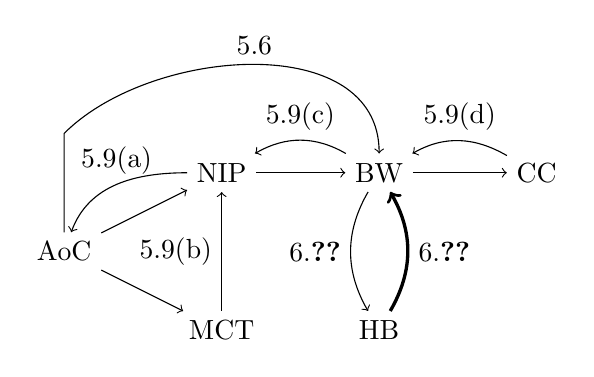
\begin{tikzpicture}
	
	% Draw nodes
	\node (AoC) at (0,0) {AoC};
	\node (MCT) at (2,-1) {MCT};
	\node (NIP) at (2,1) {NIP};
	\node (BW) at (4,1) {BW};
	\node (CC) at (6,1) {CC};
	\node (HB) at (4,-1) {HB};
	
	% Draw arcs, what we have proved in class or the homework
	\draw[->] (AoC) to (MCT);
	\draw[->] (AoC) to (NIP);
	\draw[->] (NIP) to (BW);
	\draw[->,in=90] (AoC) |- (0,1.5) to node[midway,above] {5.6} (BW);
	\draw[->] (BW) to (CC);
	\draw[->,out=180,in=70] (NIP) to node[midway,above] {5.9(a)} (AoC);
	\draw[->] (MCT) to node[midway,left] {5.9(b)} (NIP);
	\draw[->,out=150,in=30] (BW) to node[midway,above] {5.9(c)} (NIP);
	\draw[->,out=150,in=30] (CC) to node[midway,above] {5.9(d)} (BW);
	
	% Draw arcs, what we will prove here
	\draw[->,out=-120,in=120] (BW) to node[midway,left] {6.\ref{prob:BW-HB}} (HB);
	\draw[->,very thick,out=60,in=-60] (HB) to node[midway,right] {6.\ref{prob:HB-BW}}  (BW);
	
	\end{tikzpicture}
	\caption{A directed graph showing the logical implications of the various statements.}\label{fig:theorems}
	\end{center}
	\end{figure}
	
	%%%%%%%%%
	
The Bolzano-Weiestrass Theorem is often stated as: Every bounded infinite set of real numbers has at least one limit point.

We can see the connection with our statement that every bounded sequence has a convergent subsequence by considering the proof that we did in class.  We take our bounded infinite set, and we place it inside an interval, $[-M,M]$.  We then create new subintervals by bisecting the previous intervals.  We then use the end points to create a sequence, which converges to a number.  This number is then the limit point of our bounded infinite set.  So the two ideas are equivalent.

We will use the Heine-Borel Theorem to prove this alternate version of the Bolzano-Weierstrass Theorem.  We will also use the open cover version of compactness.

Prove that if $A \subseteq \mathbb{R}$ is a bounded infinite set, then $A$ has at least one limit point.  Hint: use proof by contradiction.  Build an open cover of a closed interval that contains $A$, and then use a finite subcover to show that $A$ must be finite.

	
%%%%%%%%%%%%%

\end{enumerate}

\end{document}
